\chapter{Theoretical Background}
\label{Theoretical Background}

\section*{Generative Adversarial Nets}

Generative Adversarial Networks (GANs) consist of a generator G and a discriminator D, 
both implemented using artificial neural networks. The parametrization of GANs involves 
defining the network structure of these components and initializing their weights and biases \citep{10.1007/s10928-021-09787-4}. 
The success of GANs relies on balancing the training of these two networks, where the 
G aims to produce samples $G(z)$ that mimic real data distributions $p_{data}(x)$ by input noise z, while the D 
learns to differentiate between real and generated samples \citep{10.1109/taslp.2017.2761547}. 
The training process involves iteratively updating the weights and biases of the networks through 
adversarial training, where the generator tries to deceive the discriminator, and the discriminator 
aims to accurately classify samples \citep{10.48550/arxiv.1802.05637}.

\begin{equation}
    \min_{G} \max_{D} V(D, G) = \mathbb{E}_{x \sim p_{data}(x)} [\log D(x)] + \mathbb{E}_{z \sim p_{z}(z)} [\log(1 - D(G(z)))].
\end{equation}


The formula 3.1 is the objective function of Generative Adversarial Networks (GANs). 
It describes the game process between the Generator (G) and the Discriminator (D). Specifically, the formula defines a minimax game between the Discriminator and the Generator.

\begin{itemize}
    \item \textbf{ $D(G(z))$:} is the output of the discriminator for the data G(z) generated by the generator. Indicating the probability that the discriminator believes that the generated data comes from the real data distribution.
    \item \textbf{$D(x)$:} is the output of the discriminator for the real data x. Indicating the probability that the discriminator believes that the real data x comes from the real data distribution.
    \item \textbf{ $x \sim p_{data}(x)$:} means that sample x is drawn from the true data distribution $p_{data}$.
    \item \textbf{ $z \sim p_{z}(z)$:} means that sample z is drawn from the fake data distribution $p_{z}$.
    \item \textbf{$\mathbb{E}{_x \sim p_{data}(x)}[\log D(x)]$:} means taking the average value of $\log D(x)$ for all samples x on the true data distribution $p_{data}(x)$.
    \item \textbf{$\mathbb{E}{x \sim p_{z}(z)}[\log (1 - D(x))]$:} means taking the average value of $\log (1 - D(G(z)))$ for all samples z on the noise distribution $p_z(z)$.
\end{itemize}




D(G(z)) is the output of the discriminator for the data G(z) generated by the generator, 
indicating the probability that the discriminator believes that the generated data comes from the real data distribution.
D(x) is the output of the discriminator for the real data x, 
indicating the probability that the discriminator believes that the real data x comes from the real data distribution.

$\mathbb{E}{x \sim p_{data}(x)}[\log D(x)]$ represents the average value of $\log D(x)$ for all samples x on the true data distribution $p_{data}(x)$.
$x \sim p_{data}(x)$ means that sample x is drawn from the true data distribution $p_{data}$.
$\log D(x)$ is the logarithm of the output of the discriminator D for the input x.


\begin{equation}
    \max_{D} V(D, G) = \mathbb{E}_{x \sim p_{data}(x)} [\log D(x)] + \mathbb{E}_{z \sim p_{z}(z)} [\log(1 - D(G(z)))].
\end{equation}

The formula 3.2 shows, the discriminator tries to maximize V(D, G).

\begin{equation}
    \min_{G} V(D, G) = \mathbb{E}_{z \sim p_{z}(z)} [\log(1 - D(G(z)))].
\end{equation}


The formula 3.3 shows, the generator tries to minimize V(D, G). 
This means that the generator tries to generate realistic data G(z) so that the discriminator cannot distinguish 
them from real data, that is: It is hoped that D(G(z)) is close to 1, so that $\log (1 - D(G(z)))$ is closer to negative infinity.
This dynamic equilibrium drives the GAN framework towards generating outputs that closely resemble authentic data, 
fulfilling the objective of producing realistic data that is challenging to distinguish from real data.


\begin{equation}
    \min_{G} V(D, G) = \mathbb{E}_{z \sim p_{z}(z)} [-\log(D(G(z)))].
\end{equation}

In real training process, the formula 3.3 will replace by 3.4. Since, when the discriminator D is strong, 
the gradient of the $log(1 - D(G(z)))$ approaches zero, leading to slow generator training and diminished gradient update impact \citep{10.1007/s11263-019-01265-2}.  
This approach ensures that the gradient of the logarithm is large, providing the generator with more effective gradient updates and 
helping to avoid the vanishing gradient issue \citep{10.1109/tpami.2018.2872043}.



The GAN network parameters play a crucial role in determining the quality and diversity of 
the generated samples $G(x)$ \citep{10.1007/s10928-021-09787-4}. The optimization process in GANs 
typically involves minimizing a min-max function to ensure the G produces samples that 
are indistinguishable from real data \citep{10.1109/taslp.2017.2761547}. Maintaining this balance 
during training is essential for achieving high-quality sample generation \citep{10.1007/s10928-021-09787-4}. 
The D's role is to provide feedback to the generator by acting as a critic, 
guiding the G towards producing more realistic samples \citep{10.48550/arxiv.1802.05637}.



\section*{Theoretical Results}

The training process of Generative Adversarial Networks (GANs) is inherently adversarial. 
The generator endeavors to create increasingly realistic fake samples to deceive the discriminator, 
while the discriminator seeks to more accurately distinguish between real and fake samples. 
To understand how this process works, in the following sections, 
I will describe the GAN training process from the perspectives of data distribution and mathematical formulation.

\subsection*{Distribution}



\begin{figure}[H]
    \centering
    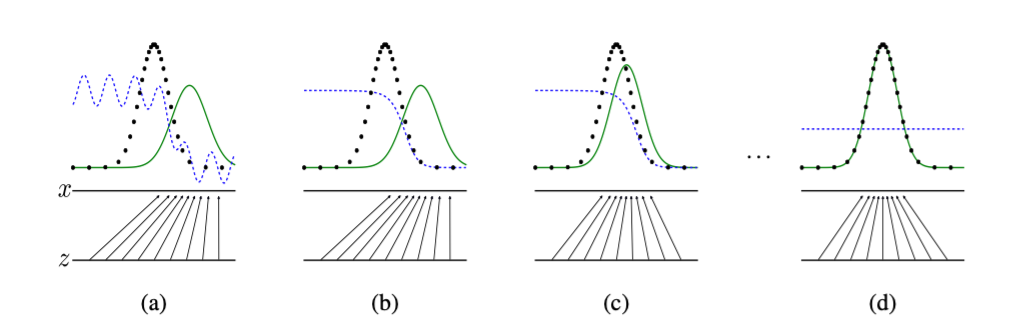
\includegraphics[width=1.2\linewidth]{./Images/data_distribution.jpg}
    \caption{Diagram of GAN training process}
    \label{fig:my_picture}
    \vspace{1pt} % Vertical space, optional
    \small{Source: \cite{goodfellow2014generative}}
\end{figure}